\documentclass[compress]{beamer}

\usetheme[block=fill]{metropolis}

\usepackage{graphicx} % Allows including images
\usepackage{amsmath,amsfonts,amsthm,amssymb}
\usepackage{color}
\usepackage{xcolor,cancel}
\usepackage{enumitem}
\setitemize{label=\usebeamerfont*{itemize item}%
	\usebeamercolor[fg]{itemize item}
	\usebeamertemplate{itemize item}}
\definecolor{mDarkBrown}{HTML}{604c38}
\definecolor{mDarkTeal}{HTML}{23373b}
\definecolor{mLightBrown}{HTML}{EB811B}
\definecolor{mMediumBrown}{HTML}{C87A2F}
\definecolor{mygreen}{HTML}{98C2B9}
\definecolor{myyellow}{HTML}{DFD79C}
\definecolor{myblue}{HTML}{8CA7CC}
\definecolor{kern}{HTML}{8CC2B7}


\usepackage{float}
\usepackage{framed}
\usepackage{epsfig}
\usepackage{graphicx}
\usepackage{subcaption}
\usepackage{ulem}
\usepackage{hhline}
\usepackage{multirow}
\usepackage{comment}   
\usepackage{bbm}
\usepackage{tikz}   
\def\Put(#1,#2)#3{\leavevmode\makebox(0,0){\put(#1,#2){#3}}}
\newcommand*\mystrut[1]{\vrule width0pt height0pt depth#1\relax}
\newcommand{\eqdef}{\mathbin{\stackrel{\rm def}{=}}}


\newcommand{\bs}[1]{\boldsymbol{#1}}
\newcommand{\bv}[1]{\mathbf{#1}}
\newcommand{\R}{\mathbb{R}}
\newcommand{\E}{\mathbb{E}}

\DeclareMathOperator*{\argmin}{arg\,min}
\DeclareMathOperator*{\argmax}{arg\,max}
\DeclareMathOperator{\nnz}{nnz}
\DeclareMathOperator{\Var}{Var}
\DeclareMathOperator{\sinc}{sinc}
\DeclareMathOperator{\sign}{sign}
\DeclareMathOperator{\dist}{dist}
\DeclareMathOperator{\mv}{mv}
\DeclareMathOperator{\sgn}{sgn}
\DeclareMathOperator{\step}{step}
\DeclareMathOperator{\gap}{gap}
\DeclareMathOperator{\poly}{poly}
\DeclareMathOperator{\tr}{tr}
\DeclareMathOperator{\orth}{orth}
\newcommand{\norm}[1]{\|#1\|}
\captionsetup[subfigure]{labelformat=empty}
\captionsetup[figure]{labelformat=empty}
\DeclareMathOperator*{\lmin}{\lambda_{min}}
\DeclareMathOperator*{\lmax}{\lambda_{max}}

\newcommand{\specialcell}[2][c]{%
  \begin{tabular}[#1]{@{}c@{}}#2\end{tabular}}
\newcommand{\specialcellleft}[2][c]{%
\begin{tabular}[#1]{@{}l@{}}#2\end{tabular}
}

\newtheorem{claim}[theorem]{Claim}
%\newtheorem{corollary}[theorem]{Corollary}

\usepackage{tabstackengine}
\stackMath


%----------------------------------------------------------------------------------------
%	TITLE PAGE
%----------------------------------------------------------------------------------------

\title{CS-GY 9223 I: Lecture 6 \\ Smoothness, Strong convexity, and more.}
\author{NYU Tandon School of Engineering, Prof. Christopher Musco}
\date{}

\begin{document}

\begin{frame}
	\titlepage 
\end{frame}

\metroset{titleformat=smallcaps}

\begin{frame}[t]
	\frametitle{gradient descent analysis}
	\textbf{Assume:}
	\begin{itemize}
		\item $f$ is convex.
		\item Lipschitz function: for all $\bv{x}$, $\|\nabla f(\bv{x})\|_2 \leq \alert{G}$.
		\item Starting radius: $\|\bv{x}^{*} - \bv{x}^{(1)}\|_2 \leq \alert{R}$.
	\end{itemize}
	
	\textbf{Gradient descent:}
	\begin{itemize}
		\item Choose number of steps $T$.
		\item $\eta = \frac{R}{G\sqrt{T}}$
		\item For $i = 1,\ldots, T$:
		\begin{itemize}
			\item $\bv{x}^{(i+1)} = \bv{x}^{(i)} - \eta \nabla f(\bv{x}^{(i)})$
		\end{itemize}
		\item Return $\hat{\bv{x}} = \argmin_{\bv{x}^{(i)}} f(\bv{x}^{(i)})$.
	\end{itemize}
	\begin{theorem}[GD Convergence Bound]
	If $T \geq \frac{R^2G^2}{\epsilon^2}$, then $f(\hat{\bv{x}}) \leq f(\bv{x}^*) + \epsilon$.
	\end{theorem}
\end{frame}

\begin{frame}
	\frametitle{online gradient descent}
	Instead of a single function $f$ to minimize, assume we have an unknown and changing set of objective functions:
	\begin{align*}
	f_1, \ldots, f_T.
	\end{align*}
	\begin{itemize}
	\item At each time step, choose $\bv{x}^{(i)}$.
	\item $f_i$ is revealed and we pay cost $f_i(\bv{x}^{(i)})$
	\item \textbf{Goal}: Minimize $\sum_{i=1}^T f_i(\bv{x}^{(i)})$. 
	\end{itemize}
\end{frame}

\begin{frame}
	\frametitle{example}
	\textbf{Email spam filtering:}
	\begin{center}
		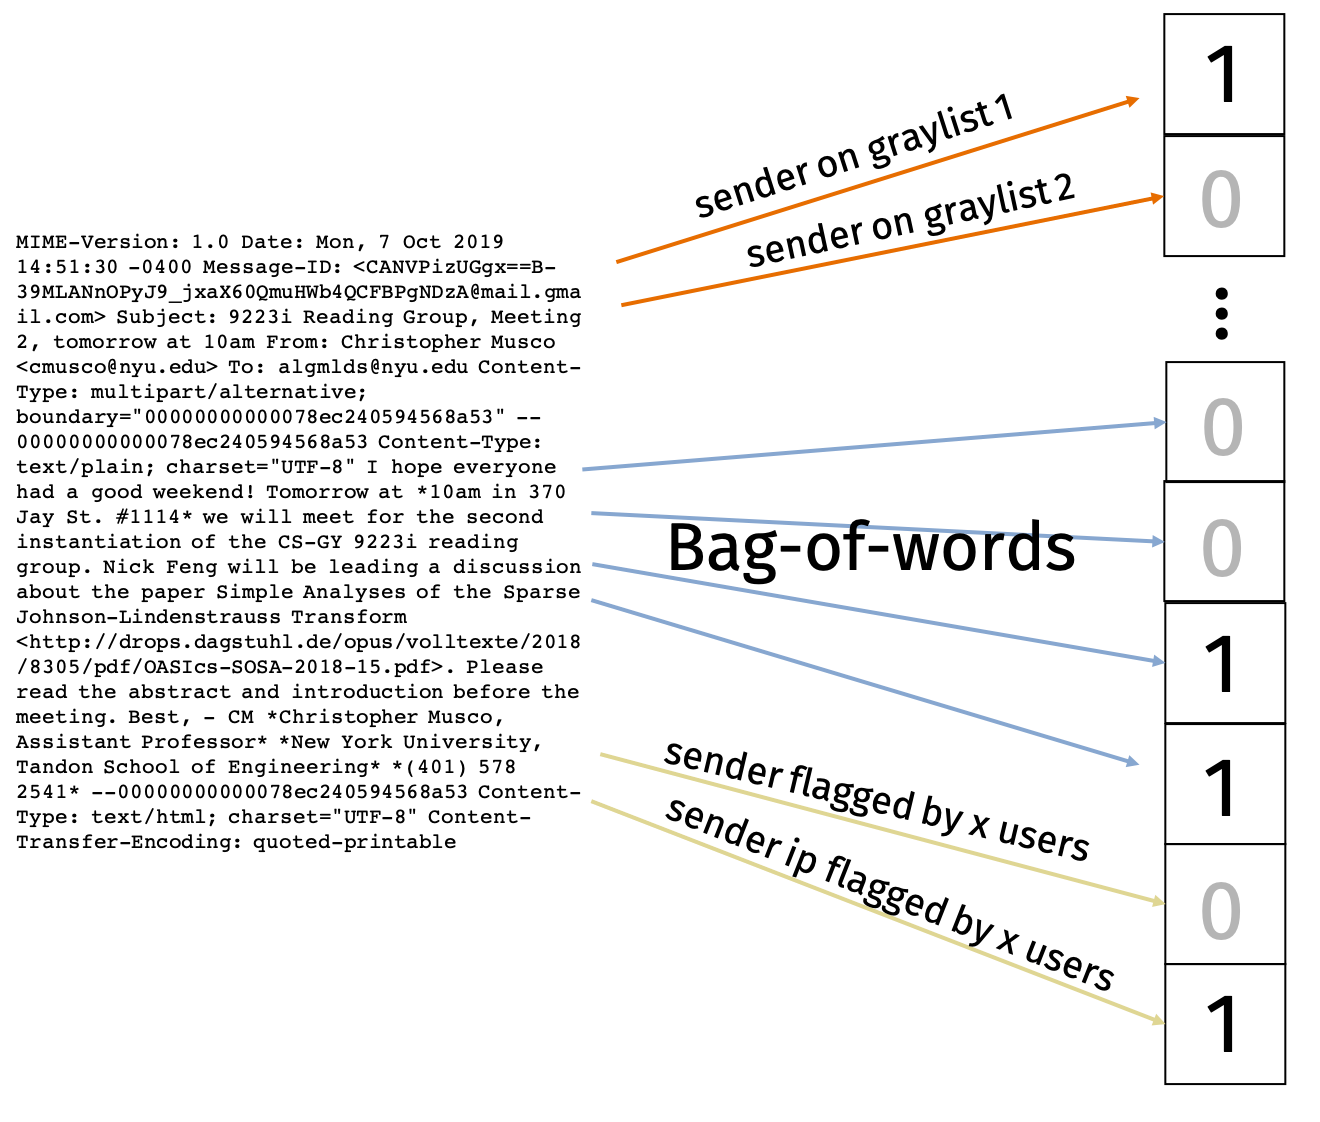
\includegraphics[width=.7\textwidth]{spam_features.png}
	\end{center}
\end{frame}

\begin{frame}
	\frametitle{spam filtering}
	\begin{itemize}
		\item $M_{\bv{x}}(\bv{y}) = \frac{1}{1 + e^{-\bv{x}^T\bv{y}}}$
	\end{itemize}
	\begin{center}
		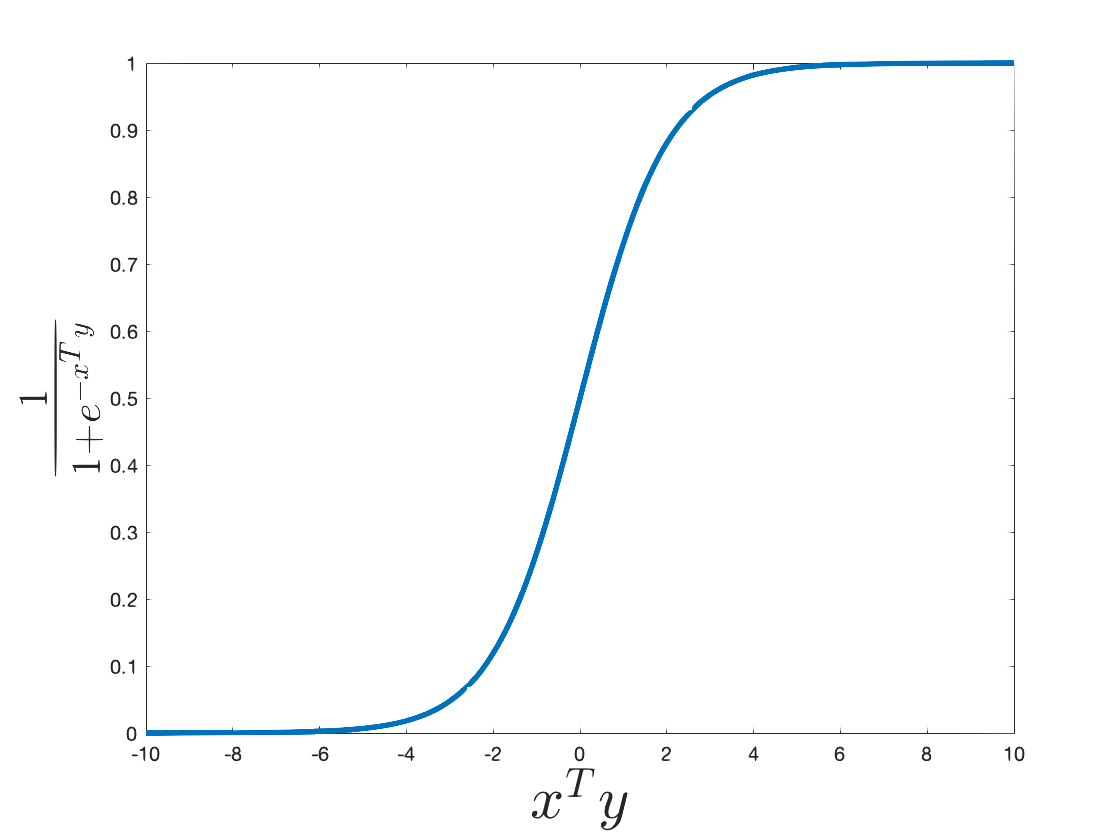
\includegraphics[width=.7\textwidth]{logistic_link.png}
	\end{center}
	Predict $\bv{y}$ as spam if $M_{\bv{x}}(\bv{y}) \geq \frac{1}{2}$.
\end{frame}

\begin{frame}
	\frametitle{spam filtering}
	\textbf{Logistic loss:}
	
	Given label $b\in \{0,1\}$,
	\begin{align*}
		L(b, M_{\bv{x}}(\bv{y})) = -b \log\left(M_{\bv{x}}(\bv{y})\right) + (1-b)\log\left(1 - M_{\bv{x}}(\bv{y})\right)
	\end{align*}
	
	\textbf{Total cost of over time:}
	\begin{align*}
	\sum_{i=1}^T L(b^{(i)}, M_{\bv{x}^{(i)}}(\bv{y}^{(i)}))) 
	\end{align*}
	where $\bv{y}^{(i)}$ is the $i^\text{th}$ email and  $b^{(i)}$ is the $i^\text{th}$ label. 
\end{frame}

\begin{frame}[t]
	\frametitle{regret bound}
	\textbf{How should we measure how well we did?}
	
	For some small value $\Delta$, can we achieve:
	\begin{align*}
	\sum_{i=1}^T f_i(\bv{x}^{(i)}) \leq \left[\min_\bv{x} \sum_{i=1}^T f_i(\bv{x})\right] + \Delta.
	\end{align*}
	I.e. can we compete  with the best \emph{fixed} solution in hindsight.
	\begin{center}
		$\Delta$ = ``regret''
	\end{center}
\end{frame}

\begin{frame}[t]
	\frametitle{online gradient descent}
	\textbf{Assume:}
	\begin{itemize}
		\item Lipschitz functions: for all $\bv{x}$, $i$, $\|\nabla f_i(\bv{x})\|_2 \leq \alert{G}$.
		\item Starting radius: $\|\bv{x}^{*} - \bv{x}^{(1)}\|_2 \leq \alert{R}$.
	\end{itemize}
	
	\textbf{Online Gradient descent:}
	\begin{itemize}
		\item Choose number of steps $T$.
		\item $\eta = \frac{D}{G\sqrt{T}}$
		\item For $i = 1,\ldots, T$:
		\begin{itemize}
			\item $\bv{x}^{(i+1)} = \bv{x}^{(i)} - \eta \nabla f_i(\bv{x}^{(i)})$
		\end{itemize}
		\item Play $\bv{x}^{(i+1)}$. 
	\end{itemize}
	\begin{claim}[OGD Regret Bound]
	After $T$ steps, $\Delta = \left[\sum_{i=1}^T f_i(\bv{x}^{(i)})\right] - \left[\sum_{i=1}^T f_i(\bv{x}^*)\right] \leq RG\sqrt{T}$
	\end{claim}
\end{frame}

\begin{frame}[t]
	\frametitle{stochastic gradient descent}
	Recall the machine learning setup. In empirical risk minimization, we can typically write:
	\begin{align*}
	f(\bv{x}) = \sum_{j=1}^n f_j(\bv{x})
	\end{align*}
	where $f_i$ is the loss function for a particular data point.
	\vspace{1em}
	
	\textbf{Linear regression:}
	\begin{align*}
		f(\bv{x}) = \sum_{j=1}^n (\bv{x}^T\bv{y}^{(j)} - b^{(j)})^2
	\end{align*}
\end{frame}

\begin{frame}
	\frametitle{stochastic gradient descent}
	\textbf{Pick random $j \in 1, \ldots, n$}:
	\begin{align*}
	\E\left[\nabla f_j(\bv{x})\right] = \nabla f(\bv{x}).
	\end{align*}
	But $\nabla f_j(\bv{x})$ can often be computed in a $1/n$ fraction of the time!
	
	\vspace{3em}
	{\textbf{Main idea:} Use random approximate gradient in place of actual gradient.}
	
	\begin{center}
	 	\alert{\textbf{Trade slower convergence for cheaper iterations.}}
	 \end{center}
\end{frame}

\begin{frame}[t]
	\frametitle{stochastic gradient descent}
	\textbf{Assume:}
	\begin{itemize}
		\item Lipschitz functions: for all $\bv{x}$, $j$, \alert{$\|\nabla f_j(\bv{x})\|_2 \leq \frac{G'}{n}$.}
		\item Starting radius: \alert{$\|\bv{x}^{*} - \bv{x}^{(1)}\|_2 \leq R$.}
	\end{itemize}
	
	\textbf{Stochastic Gradient descent:}
	\begin{itemize}
		\item Choose number of steps $T$.
		\item $\eta = \frac{D}{G'\sqrt{T}}$
		\item For $i = 1,\ldots, T$:
		\begin{itemize}
			\item Pick random $j_i \in 1, \ldots, n$.
			\item $\bv{x}^{(i+1)} = \bv{x}^{(i)} - \eta \nabla f_{j_i}(\bv{x}^{(i)})$
		\end{itemize}
		\item Return $\hat{\bv{x}} = \frac{1}{T}\sum_{i=1}^T \bv{x}^{(i)}$
	\end{itemize}
\end{frame}

\begin{frame}[t]
\frametitle{visualizing SGD}
\begin{center}
	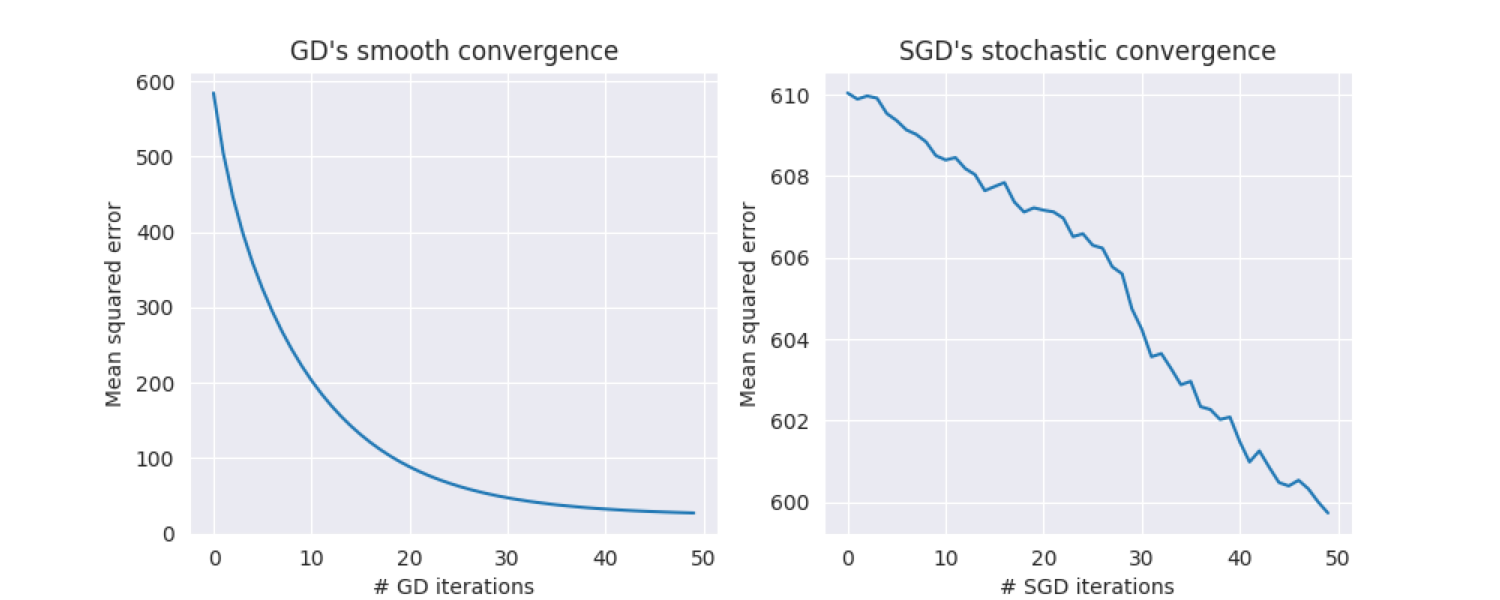
\includegraphics[height=.35\textheight]{gd_convergence.png}
	
	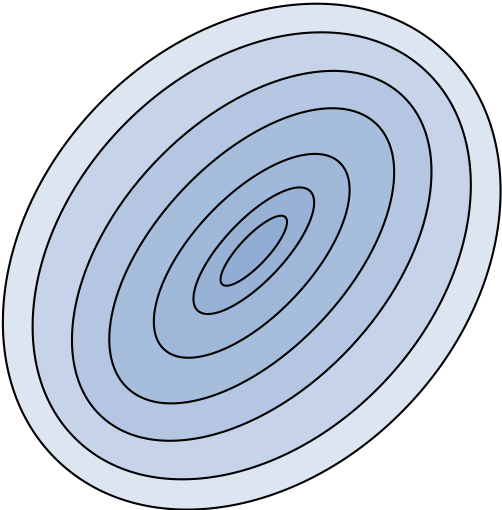
\includegraphics[height=.5\textheight]{gd_paths_raw.png}
\end{center}	
\end{frame}

\begin{frame}[t]
	\frametitle{stochastic gradient descent analysis}
	\begin{claim}[SGD Convergence]
		After $T = \frac{R^2G'^2}{\epsilon^2}$ iterations:
		\begin{align*}
			\E\left[f(\hat{\bv{x}}) - f(\bv{x}^*)\right] \leq \epsilon.
		\end{align*}
	where $\hat{\bv{x}} = \frac{1}{T}\sum_{i=1}^T \bv{x}^{(i)}$.
	\end{claim}
\textbf{Claim 1:} 
\begin{align*}
	f(\hat{\bv{x}}) - f(\bv{x}^*) \leq \frac{1}{T}\left[f(\bv{x}^{(i)}) -f(\bv{x}^*)\right]
\end{align*}
\end{frame}

\begin{frame}[t]
	\frametitle{stochastic gradient descent analysis}
	\begin{claim}[SGD Convergence]
		After $T = \frac{R^2G'^2}{\epsilon^2}$ iteration:
		\begin{align*}
		\E\left[f(\hat{\bv{x}}) - f(\bv{x}^*)\right] \leq \epsilon.
		\end{align*}
	\end{claim}
\end{frame}

\begin{frame}[t]
	\frametitle{comparison}
	Number of iterations for error $\epsilon$:
	\begin{itemize}
		\item \textbf{Gradient Descent}: $T = \frac{R^2 G^2}{\epsilon^2}$. 
		\item \textbf{Stochastic Gradient Descent}: $T = \frac{R^2 G'^2}{\epsilon^2}$. 
	\end{itemize}

	\textbf{Always have $G \leq G'$:}
	\begin{align*}
		\|\nabla f(x)\|_2 \leq \|\nabla f_1(x)\|_2 + \ldots + \|\nabla f_n(x)\|_2 \leq n\cdot\frac{G'}{n} = G'.
	\end{align*}
	
	\textbf{Fair comparison:}
	\begin{itemize}
		\item SGD cost = $(\# \text{ of iterations})\cdot O(1)$
		\item GD cost = $(\# \text{ of iterations})\cdot O(n)$
	\end{itemize}
\end{frame}

\begin{frame}[t]
	\frametitle{comparison}
	\textbf{Stochastic vs. Full Batch Gradient Descent:}
\end{frame}

\begin{frame}
	\frametitle{beyond the basic bound}
	Can the convergence bounds be tightened for certain functions? Can they guide us towards faster algorithms?
	
	\textbf{Goals:}
	\begin{itemize}
		\item Improve $\epsilon$ dependence below $1/\epsilon^2$.
		\item Reduce or eliminate dependence on $G$ and $R$.
		\item Etc. 
	\end{itemize}
\end{frame}

\begin{frame}[t]
	\frametitle{smoothness}
	\begin{definition}[$\beta$-smoothness]
	A function $f$ is $\alert{\beta}$ smooth if, for all $\bv{x}$, $\bv{y}$
	\begin{align*}
		\|\nabla f(\bv{x}) - \nabla f(\bv{y})\|_2 \leq \alert{\beta} \|\bv{x} - \bv{y}\|_2
	\end{align*}
	\end{definition}
	$\beta$ is a parameter that will depend on our function.
\end{frame}

\begin{frame}[t]
	\frametitle{smoothness}
	Recall from definition of convexity that:
	\begin{align*}
	f(\bv{x}) - f(\bv{y}) \leq \nabla f(\bv{x})^T(\bv{x} - \bv{y})
	\end{align*}
	\begin{center}
		\alert{How much smaller can left hand side be?}
	\end{center}
	\begin{align*}
		\nabla f(\bv{x})^T(\bv{x} - \bv{y}) - \left[f(\bv{x}) - f(\bv{y})\right] \leq \frac{\beta}{2}\|\bv{x} - \bv{y}\|_2^2
	\end{align*}
\end{frame}

\begin{frame}[t]
	\frametitle{guaranteed progress}
	Previously learning rate/step size $\eta$ depended on $G$. Now choose it based on $\beta$:
	\begin{align*}
	\bv{x}^{(t+1)} \leftarrow \bv{x}^{(t)} - \frac{1}{\beta}\nabla f(\bv{x}^{(t)})
	\end{align*}
	
	\textbf{Progress per step of gradient descent:}
\end{frame}

\begin{frame}[t]
	\frametitle{convergence guarantee}
	\begin{theorem}[GD convergence for $\beta$-smooth functions.]
		Let $f$ be a \alert{$\beta$} smooth convex function and assume we have $\|\bv{x}^{*} - \bv{x}^{(1)}\|_2 \leq \alert{R}$. If we run GD for $T$ steps with $\eta = \frac{1}{\beta}$ we have:
		\begin{align*}
		f(\bv{x}^{(T)}) - f(\bv{x}^*) \leq \frac{2\beta R^2}{T-1} 
		\end{align*} 
	\end{theorem}
	\textbf{Corollary}: If \alert{$T = O\left(\frac{\beta R^2}{\epsilon}\right)$} we have $f(\bv{x}^{(T)}) - f(\bv{x}^*) \leq \epsilon$.
\end{frame}

\begin{frame}[t]
	\frametitle{strong convexity}
	\begin{definition}[$\alpha$-strongly convex]
		A convex function $f$ is $\alert{\alpha}$-strongly convex if, for all $\bv{x}$, $\bv{y}$
		\begin{align*}
		f(\bv{y}) \geq f(\bv{x}) + \nabla f(\bv{x})^T(\bv{y} - \bv{x}) + \frac{\alpha}{2} \|\bv{x} - \bv{y}\|_2^2
		\end{align*}
	\end{definition}
	$\alpha$ is a parameter that will depend on our function.
\end{frame}

\begin{frame}[t]
	\frametitle{strong convexity}
	\textbf{Completing the picture:}
	If $f$ is $\alpha$ strongly convex and $\beta$ smooth,
	\begin{align*}
	\alert{\frac{\alpha}{2}}\|\bv{x} - \bv{y}\|_2^2 \leq \nabla f(\bv{x})^T(\bv{x} - \bv{y}) - \left[f(\bv{x}) - f(\bv{y})\right] \leq \alert{\frac{\beta}{2}}\|\bv{x} - \bv{y}\|_2^2.
	\end{align*}
\end{frame}

\begin{frame}[t]
	\frametitle{gd for strongly convex function}
	\textbf{Gradient descent for strongly convex functions:}
	\begin{itemize}
		\item Choose number of steps $T$.
		\item For $i = 1,\ldots, T$:
		\begin{itemize}
			\item $\eta = \frac{2}{\alpha\cdot(i+1)}$
			\item $\bv{x}^{(i+1)} = \bv{x}^{(i)} - \eta \nabla f(\bv{x}^{(i)})$
		\end{itemize}
		\item Return $\hat{\bv{x}} = \argmin_{\bv{x}^{(i)}} f(\bv{x}^{(i)})$. 
		\item Alternatively, return $\hat{\bv{x}} = \sum_{i=1}^T \frac{2i}{T(T+1)} \bv{x}^{(i)}$.
	\end{itemize}
\end{frame}

\begin{frame}[t]
	\frametitle{convergence guarantee}
	\begin{theorem}[GD convergence for $\alpha$-strongly convex functions.]
		Let $f$ be an \alert{$\alpha$}-strongly convex function and assume we have that, for all $\bv{x}$, $\|\nabla f(\bv{x})\|_2 \leq \alert{G}$. If we run GD for $T$ steps (with adaptive step sizes) we have:
		\begin{align*}
		f(\hat{\bv{x}}) - f(\bv{x}^*) \leq \frac{2G^2}{\alpha(T-1)} 
		\end{align*} 
	\end{theorem}
	\textbf{Corollary}: If \alert{$T = O\left(\frac{G^2}{\alpha \epsilon}\right)$} we have $f(\hat{\bv{x}}) - f(\bv{x}^*) \leq \epsilon$
\end{frame}


\begin{frame}[t]
	\frametitle{smooth and strongly convex}
	\begin{center}
	What if $f$ is both $\beta$-smooth and $\alpha$-strongly convex?
	\end{center}
	\begin{align*}
	\alert{\frac{\alpha}{2}}\|\bv{x} - \bv{y}\|_2^2 \leq \nabla f(\bv{x})^T(\bv{x} - \bv{y}) - \left[f(\bv{x}) - f(\bv{y})\right] \leq \alert{\frac{\beta}{2}}\|\bv{x} - \bv{y}\|_2^2.
	\end{align*}
	
	\textbf{What if $\alpha = \beta$:}
	
\end{frame}

\begin{frame}[t]
	\frametitle{smooth and strongly convex}
	\begin{center}
		What if $f$ is both $\beta$-smooth and $\alpha$-strongly convex?
	\end{center}
	\begin{align*}
	\alert{\frac{\alpha}{2}}\|\bv{x} - \bv{y}\|_2^2 \leq \nabla f(\bv{x})^T(\bv{x} - \bv{y}) - \left[f(\bv{x}) - f(\bv{y})\right] \leq \alert{\frac{\beta}{2}}\|\bv{x} - \bv{y}\|_2^2.
	\end{align*}
	
	\textbf{What if $\alpha = \beta$:}
\end{frame}

\begin{frame}[t]
	\frametitle{convergence guarantee}
	\begin{theorem}[GD for $\beta$-smooth, $\alpha$-strongly convex.]
		Let $f$ be a $\beta$-smooth and $\alpha$-strongly convex function. If we run GD for $T$ steps (with step size $\eta = \frac{1}{\beta}$) we have:
		\begin{align*}
		\|\bv{x}^{(t)} - \bv{x}^*\|_2^2 \leq e^{-(t-1)\frac{\alpha}{\beta}} \|\bv{x}^{(1)} - \bv{x}^*\|_2^2
		\end{align*} 
	\end{theorem}	
	\begin{center}
		\alert{$\kappa = \frac{\beta}{\alpha}$} is called the ``condition number'' of $f$. 
		
		\textbf{Is it better if $\kappa$ is large or small?}
	\end{center}
\end{frame}

\begin{frame}[t]
	\frametitle{smooth and strongly convex}
	\textbf{Converting to more familiar form:}
	\begin{align*}
	\alert{\frac{\alpha}{2}}\|\bv{x} - \bv{y}\|_2^2 \leq \nabla f(\bv{x})^T(\bv{x} - \bv{y}) - \left[f(\bv{x}) - f(\bv{y})\right] \leq \alert{\frac{\beta}{2}}\|\bv{x} - \bv{y}\|_2^2.
	\end{align*}	
\end{frame}

\begin{frame}[t]
	\frametitle{convergence guarantee}
	\begin{corollary}[GD for $\beta$-smooth, $\alpha$-strongly convex.]
		Let $f$ be a $\beta$-smooth and $\alpha$-strongly convex function. If we run GD for $T$ steps (with step size $\eta = \frac{1}{\beta}$) we have:
		\begin{align*}
		f(\bv{x}^{(t)}) - f(\bv{x}^*)  \leq \frac{\beta}{2} e^{-(t-1)\frac{\alpha}{\beta}} R
		\end{align*} 
	\end{corollary}	
	\textbf{Corollary}: 
	If \alert{$T = O\left(\frac{\beta}{\alpha}\log(\beta R/ \epsilon)\right)$} we have:
	\begin{align*}
	f(\hat{\bv{x}}) - f(\bv{x}^*) \leq \epsilon.
	\end{align*}
	
	\textbf{Alternative}: 
	If \alert{$T = O\left(\frac{\beta}{\alpha}\log(\beta/\alpha \epsilon)\right)$} we have:
	\begin{align*}
	f(\hat{\bv{x}}) - f(\bv{x}^*) \leq \epsilon \left[f(\bv{x}^{(1)}) - f(\bv{x}^*)\right]
	\end{align*}

\end{frame}

\begin{frame}[t]
	\frametitle{understanding conditioning}
	Let $f(\bv{x}) = \|\bv{D}\bv{x} - \bv{b}\|_2^2$ where $\bv{D}$ is a diagaonl matrix. For now imagine we're in two dimensions: $\bv{x} = \begin{bmatrix}
	x_1\\
	x_2
	\end{bmatrix}$, $\bv{D} = \begin{bmatrix}
	d_1 & 0 \\
	0 & d_2
	\end{bmatrix}
	$.
\end{frame}

\begin{frame}[t]
	\frametitle{understanding conditioning}
	\begin{center}
	\textbf{What is $\beta$ for $f(\bv{x}) = \|\bv{D}\bv{x} - \bv{b}\|_2^2$}?
	\end{center}
		
	\textbf{In other words:} What is smallest $\beta$ so that for all $\bv{x}, \bv{y}$,
	\begin{align*}
		\|\nabla f(\bv{x}) - \nabla f(\bv{y})\|_2 \leq \beta \|\bv{x} - \bv{y}\|_2
	\end{align*}
\end{frame}

\begin{frame}[t]
	\frametitle{understanding conditioning}
	\begin{center}
		\textbf{What is $\alpha$ for $f(\bv{x}) = \|\bv{D}\bv{x} - \bv{b}\|_2^2$}?
	\end{center}
	
	\textbf{In other words:} What is largest $\alpha$ so that for all $\bv{x}, \bv{y}$, 
	\begin{align*}
		{\frac{\alpha}{2}}\|\bv{x} - \bv{y}\|_2^2 \leq \nabla f(\bv{x})^T(\bv{x} - \bv{y}) - \left[f(\bv{x}) - f(\bv{y})\right] 
	\end{align*}
\end{frame}

\begin{frame}[t]
	\frametitle{understanding conditioning}
	\begin{center}
		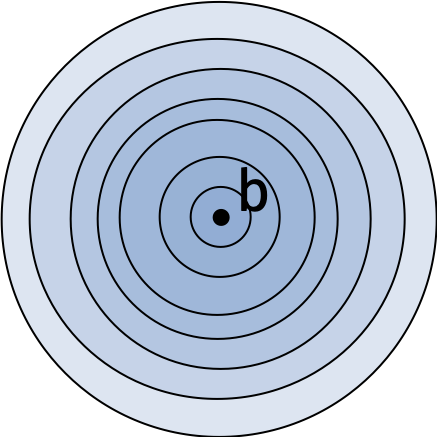
\includegraphics[width=.5\textwidth]{perfect_conditioning.png}
		
		Level sets of $\|\bv{D}\bv{x} - \bv{b}\|_2^2$ when $d_1 = 1, d_2 = 1$. 
	\end{center}
\end{frame}

\begin{frame}[t]
	\frametitle{understanding conditioning}
	\begin{center}
		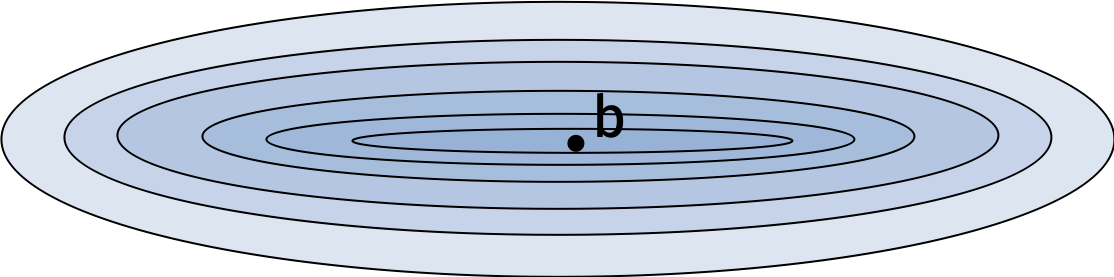
\includegraphics[width=\textwidth]{poor_conditioning.png}
		
		Level sets of $\|\bv{D}\bv{x} - \bv{b}\|_2^2$ when $d_1 = \frac{1}{3}, d_2 = 2$. 
	\end{center}
\end{frame}

\begin{frame}[t]
	\frametitle{understanding conditioning}
	Steps to convergence $\approx O\left(\kappa \log(1/\epsilon)\right) = O\left(\frac{\max(\bv{D}^2)}{\min(\bv{D}^2)}  \log(1/\epsilon)\right) $.
	
	For general regression problems $\|\bv{A}\bv{x} - \bv{b}\|_2^2$,
	\begin{align*}
		\beta = \lambda_{max}(\bv{A}^T\bv{A}) \\
		\alpha = \lambda_{min}(\bv{A}^T\bv{A})
	\end{align*}
\end{frame}


\begin{frame}[t]
	\frametitle{in-class exercise}
		\begin{theorem}[GD for $\beta$-smooth, $\alpha$-strongly convex.]
		Let $f$ be a $\beta$-smooth and $\alpha$-strongly convex function. If we run GD for $T$ steps (with step size $\eta = \frac{1}{\beta}$) we have:
		\begin{align*}
		\|\bv{x}^{(t)} - \bv{x}^*\|_2^2 \leq e^{-(t-1)\frac{\alpha}{\beta}} \|\bv{x}^{(1)} - \bv{x}^*\|_2^2
		\end{align*} 
	\end{theorem}

\begin{center}
	\alert{\textbf{Prove for $f(\bv{x}) = \|\bv{D}\bv{x} - \bv{b}\|_2^2$.}}
\end{center}	
	
\end{frame} 

\begin{frame}[t]
	\frametitle{in-class exercise}
\end{frame}

\begin{frame}[t]
	\frametitle{in-class exercise}
\end{frame}


\end{document} 








